\documentclass[reprint, english, nofootinbib]{revtex4-2}

\usepackage{graphicx}
\usepackage{subfig}
\usepackage[colorlinks=true,urlcolor=blue,citecolor=blue]{hyperref}
\usepackage{physics}
\usepackage{amsmath}
\usepackage{amssymb}
\usepackage{amsbsy}
\usepackage{bbold}

\usepackage{blindtext}
\usepackage{tikzducks}
\usepackage{listings}

\graphicspath{{../figs/}}

\begin{document}
\title{Regression analysis and resampling methods}
\author{Nicholas Karlsen}
\affiliation{University of Oslo}
\author{Thore Espedal Moe}
\affiliation{University of Oslo}
\date{\today}

\begin{abstract}
    \noindent
   In this paper we aim to explore the application of three distinct regression methods to both a sampling of the Franke function, as well as a set of terrain data. We utilize the ordinary-least-square (OLS) regression, Ridge regression and LASSO regression along with bootstrap and k-fold cross-validation re-sampling techniques in order to create and asses predictive polynomial models. We analyze the performance of the different regression models on the two data sets, with the ultimate goal of determining the best regression method and the best predictive polynomial model for each data set.
\end{abstract}

\maketitle

\section{Introduction}
    \noindent
    In essence, Linear Regression is the process of taking points from a function, or a set of measurements and mapping them to coordinates in a chosen basis in order to create an approximation, or model of the original dataset.
\section{Theory}
    See \textcite{hastie}
    \subsection{Linear Regression}
        \noindent
        Consider a set of data points $\{(x_1, y_n), \dots, (x_N, y_N)\}$ which we wish to fit to some linear model $\mathbf{\tilde y}(\pmb \beta)$ where $\pmb\beta$ is a vector containing the free parameters of the model. The model $\mathbf{\tilde y}$ will then be related to the true data points $\mathbf y$ by
        \begin{equation}
            \mathbf y = \mathbf{\tilde y}(\pmb\beta) + \pmb\varepsilon
        \end{equation}
        where $\pmb\varepsilon = (\epsilon_1, \dots, \epsilon_N)$ represents the error of the model. The aim of Linear regression models is thus to find the optimal parameters $\pmb\beta$ such that not only the error of the model on some particular dataset is minimized, but also the error of the model applied to different data sets sampled in the same domain is minimized, such that we may use our model to make predictions.

        \subsubsection{The Design Matrix}
            \noindent
            When constructing a model, we first have to chose a set of basis functions. A popular choice for which is $\mathbb P_n$, which models a wide range of different phenomena and is also the choice we will make for this paper. But in principle, any set of linear basis functions may be chosen.
            Our model will then be in the form
            \begin{equation}
                \tilde y (x) = \beta_0 + \beta_1 x + \dots \beta_n x^n
            \end{equation}
            when trying to find the optimal $\pmb \beta$, a useful quantity is the so-called Design Matrix, which for our chosen basis takes the form
            \begin{equation}
                \textup{X} = \qty[
                \begin{matrix}
                    1 & x_1 & \dots & x_1^n \\
                    1 & x_2 & \dots & x_2^n \\
                    \vdots & \vdots & \vdots & \vdots \\
                    1 & x_N & \dots & x_N^n
                \end{matrix}
                ]
            \end{equation}
            where we see that entry $\textup{X}_{ij}$ contains the $x_i$ data point evaluated in the $j$-th basis function. This matrix has the particularly useful property that we may then multiply it with $\pmb \beta$ to obtain the corresponding set of predictions $\mathbf{\tilde y}$ like
            \begin{equation}
                \mathbf{\tilde y} = \textup{X}\pmb \beta
            \end{equation}
            leaving us with a linear algebra problem to solve in finding the $\pmb\beta$ which optimizes $\mathbf{\tilde y}$.

            \begin{itemize}
                \item Scaling
            \end{itemize}

        \subsubsection{Model assessment}

        \begin{equation}
            \textup{MSE}(\mathbf y, \mathbf{\tilde y}) = \frac{1}{n}\sum_i \qty(y_i - \tilde y_i)^2
        \end{equation}
        \begin{equation}
            \textup{R}^2(\mathbf y, \tilde{\mathbf{y}}) = 1 -
            \frac{\sum_i(y_i - \tilde y_i)^2}{\sum_i \qty(y_i - \langle \mathbf y\rangle)^2}
        \end{equation}

        \subsubsection{Ordinary Least Squares}
            \noindent
            In ordinary least squares (OLS), we aim to find an optimal set of parameters $\pmb{\hat\beta} = [\hat\beta_0, \dots, \hat\beta_n]^T$ such that the $L^2$ norm $\norm{\mathbf y - \textup{X}\pmb{\beta}}_2$ is minimal, with the $L^2$ norm being induced by the inner product
            \begin{equation}
                \norm{\mathbf u}_2^2 = \sum_i u_i^2 = \mathbf u^T \mathbf u
            \end{equation}
            This defines the cost function for OLS, which may be written as
            \begin{equation}
                C_{OLS}(\pmb \beta)
                = \qty(\mathbf y - \textup{X}\pmb \beta)^T(\mathbf y - \textup{X}\pmb \beta)
            \end{equation}
            In order to find its minima, we differentiate wrt to $\pmb\beta$ and assert that $\partial_{\pmb\beta}C_{OLS} = 0$ for the optimal predictor. Taking the partial derivative yields
            \begin{align}
                \begin{split}
                \pdv{\pmb\beta}C_{OLS}(\pmb\beta) = -2\textup{X}^T\qty(\mathbf y - \textup X\pmb \beta)
                \end{split}
            \end{align}
            We assert this is zero at the minima, which yields
            \begin{equation}
                \textup{X}^T\mathbf y = \textup{X}^T\textup{X}\pmb\beta
            \end{equation}
            then taking the inverse of $\textup{X}^T\textup{X}$ on both sides then gives the optimal $\pmb\beta$ as
            \begin{equation}\label{eqn:OLS optimal beta}
                \hat{\pmb \beta}_{\textup{OLS}} = (\textup{X}^T\textup{X})^{-1}\textup{X}^T\mathbf y
            \end{equation}
            which mathematically is the best projection of the data-points to our model. However, this may not actually yield the best predictive model. OLS may suffer from over-fitting to the particular sample, and as such will not always perform very well on new data points for which the model has not been trained. As such, we instead look at alternate regression methods with additional turning parameters which allow us to account for the variance between different sets of data as to yield a model with better predictive abilities compared to the OLS.

        \subsubsection{Ridge Regression}
            \noindent
            One such method is the Ridge regression, where the cost function is given as
            \begin{equation}
                C_{R}(\pmb \beta)
                = (\mathbf y - \textup{X}\pmb\beta)^T(\mathbf y - \textup{X}\pmb\beta)
                + \lambda \pmb\beta^T\pmb\beta
            \end{equation}
			The only difference between the cost function for OLS and Ridge regression is the addition of the "penalty" parameter $\lambda$ to the $L^2$ norm of the coefficients $\pmb{\beta}$. The main point of introducing this parameter is to reduce the variance of the regression coefficients $\pmb{\beta}$. It introduces a constraint on the allowable values of $\pmb{\beta}$, which means that the method no longer is unbiased. The aim is that the reduction of the variance outweighs the increase of the method's bias, leading to an overall lower test error, cf. the later discussion of the Bias-Variance Trade-off.
        \subsubsection{Lasso Regression}
            \begin{equation}
                C_L(\pmb \beta) =
                \norm{\mathbf y - \textup{X}\pmb{\beta}}_2^2
                + \lambda\norm{\pmb{\beta}}_1
            \end{equation}
	       The Lasso method is distinguished from the Ridge regression by which norm of $\pmb{\beta}$ is penalized. While the Ridge regression applies the penalty to the $L^2$ norm, the Lasso aims to shrink the $L^1$ norm. Two important consequences arise from this: firstly, it is no longer possible to obtain a closed-form solution to the minimization problem; secondly, the regression coefficients may be shrunk far more unevenly. In contrast to the Ridge regression, Lasso regression may shrink individual $\beta_{i}$ toward zero. This is an extremely useful property of the method, since it allows unimportant predictors to be identified and discarded. The drawback, of course, is that the bias of the Lasso method is expected to exceed the bias of the Ridge method.
    \subsection{Singular Value Decomposition}
        \noindent
        Consider an $m\times n$ matrix $\textup X$ of rank $r$. The singular values of $\textup X$ are then defined as the root of the eigenvalues of the diagonal matrix $\textup X^T\textup X$. We may also express $\textup X$ in the so-called singular value decomposition (SVD)
        \begin{equation}
            \textup X = \textup{U}\Sigma\textup{V}^T
        \end{equation}
        where $\textup{U, V}$ are orthogonal matrices and
        \begin{equation}
            \Sigma =
            \qty[
            \begin{matrix}
                D & \dots & 0 \\
                \vdots & \ddots & \vdots \\
                0 & \dots & 0
            \end{matrix}
            ]
        \end{equation}
        an $m\times n$ matrix, where the matrix $\textup D$ is a diagonal $r \times r$ matrix containing the singular values of $\textup X^T \textup X$
        \begin{equation}
            D = \qty[
            \begin{matrix}
                \sigma_1 & \dots & 0 \\
                \vdots & \ddots & \vdots \\
                0 & \dots & \sigma_n
            \end{matrix}
            ]
        \end{equation}
        which by convention is ordered such that $\sigma_1 \geq \dots \geq \sigma_n$.

        \subsubsection{Application to OLS and Ridge}
            We may use the SVD to re-express the expression for $\hat{\pmb \beta}$ in OLS given by Eqn.~\ref{eqn:OLS optimal beta}
            by writing
            \begin{equation}
                \textup{X}^T\textup{X} = \qty(\textup{U}\Sigma\textup{V}^T)^T\qty(\textup{U}\Sigma\textup{V}^T)
                = \textup{V}\Sigma^T\textup{U}^T\textup{U}\Sigma\textup{V}^T
            \end{equation}
            Since $\textup{U}$ is an orthogonal matrix, it follows that $\textup{U}^T\textup{U} = \mathbb{1}$, further we have that $\Sigma^T = \Sigma$ since it is a diagonal matrix. We therefore end up with
            \begin{equation}
                \textup{X}^T\textup{X} = \textup{V}\Sigma^2\textup{V}^T
            \end{equation}
            inserting this into Eqn.~\ref{eqn:OLS optimal beta} gives us
            \begin{equation}
                \pmb{\hat{\beta}}_{\textup{OLS}} = \qty(\textup{V}\Sigma^2\textup{V}^T)^{-1} \textup{X}^T\pmb{\beta}
            \end{equation}
            we may also give a similar treatment to the Ridge regression



        \begin{itemize}
            \item Discuss problems of $X^T X$ becoming singular in OLS, and how we use SVD to work around it.
        \end{itemize}

    \subsection{Re-sampling}
        \noindent
        Re-sampling methods are ways in which we can generate new statistics from our existing data, which as the name suggests implies sampling new data sets from our already existing data. By doing so, we may gain new insights about our data which may not be available through regular analysis, particularly in situations where we are limited by the number of data points.

        Here, we will focus on two of many such techniques.

        \subsubsection{Cross Validation}
            \noindent
            In the cross-validation re-sampling method, we split our data set $S$ into $k$ equally sized subsets $s_1, \dots, s_k$.
            We then for each $i = 1,\dots, k$ assign the $i$-th subset as the test set and the remaining $k-1$ subsets as the training set and compute the statistics in the usual way. Then at the end, we compute the mean value of the $k$ sets of statistics. A visual representation of this process can be seen in Fig.~\ref{fig: Cross Validation}.
            \begin{figure}[h!tb]
                \center
                \vspace{5mm} % To avoid touching the preceding text
                \tikzset{every picture/.style={line width=0.75pt}} %set default line width to 0.75pt

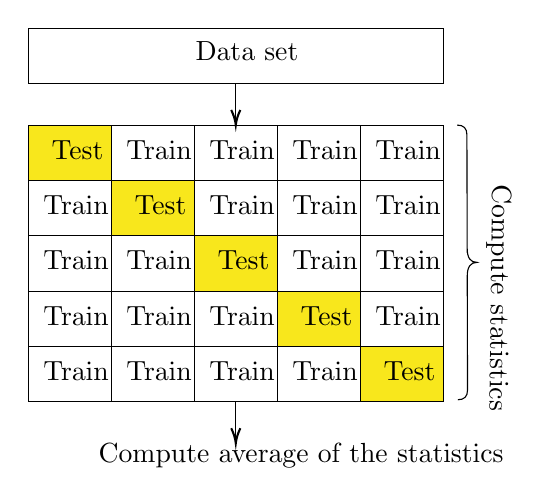
\begin{tikzpicture}[x=0.5pt,y=0.5pt,yscale=-1,xscale=1]
%uncomment if require: \path (0,487); %set diagram left start at 0, and has height of 487

%Shape: Rectangle [id:dp9628831478307318]
\draw   (90,20) -- (390,20) -- (390,60) -- (90,60) -- cycle ;
%Shape: Rectangle [id:dp40247556319098454]
\draw   (150,90) -- (210,90) -- (210,130) -- (150,130) -- cycle ;
%Straight Lines [id:da38673279994063514]
\draw    (240,60) -- (240,88) ;
\draw [shift={(240,90)}, rotate = 270] [color={rgb, 255:red, 0; green, 0; blue, 0 }  ][line width=0.75]    (10.93,-3.29) .. controls (6.95,-1.4) and (3.31,-0.3) .. (0,0) .. controls (3.31,0.3) and (6.95,1.4) .. (10.93,3.29)   ;
%Shape: Brace [id:dp44265578721237586]
\draw   (400.5,288.5) .. controls (405.17,288.49) and (407.49,286.15) .. (407.48,281.48) -- (407.28,199.23) .. controls (407.27,192.56) and (409.59,189.23) .. (414.26,189.22) .. controls (409.59,189.23) and (407.25,185.9) .. (407.23,179.23)(407.24,182.23) -- (407.03,96.98) .. controls (407.02,92.31) and (404.68,89.99) .. (400.01,90) ;
%Shape: Rectangle [id:dp6086176363319614]
\draw  [fill={rgb, 255:red, 248; green, 231; blue, 28 }  ,fill opacity=1 ] (90,90) -- (150,90) -- (150,130) -- (90,130) -- cycle ;
%Shape: Rectangle [id:dp6253670891530648]
\draw   (210,90) -- (270,90) -- (270,130) -- (210,130) -- cycle ;
%Shape: Rectangle [id:dp012463141021535118]
\draw   (270,90) -- (330,90) -- (330,130) -- (270,130) -- cycle ;
%Shape: Rectangle [id:dp03635717517805359]
\draw   (330,90) -- (390,90) -- (390,130) -- (330,130) -- cycle ;
%Shape: Rectangle [id:dp6139521323150046]
\draw   (90,130) -- (150,130) -- (150,170) -- (90,170) -- cycle ;
%Shape: Rectangle [id:dp2734748607023023]
\draw   (210,130) -- (270,130) -- (270,170) -- (210,170) -- cycle ;
%Shape: Rectangle [id:dp7416160208443594]
\draw   (270,130) -- (330,130) -- (330,170) -- (270,170) -- cycle ;
%Shape: Rectangle [id:dp04965387626199025]
\draw   (330,130) -- (390,130) -- (390,170) -- (330,170) -- cycle ;
%Shape: Rectangle [id:dp36390369464546923]
\draw   (90,170) -- (150,170) -- (150,210) -- (90,210) -- cycle ;
%Shape: Rectangle [id:dp0583337342908441]
\draw   (150,170) -- (210,170) -- (210,210) -- (150,210) -- cycle ;
%Shape: Rectangle [id:dp7518796244751725]
\draw   (270,170) -- (330,170) -- (330,210) -- (270,210) -- cycle ;
%Shape: Rectangle [id:dp8731512433065419]
\draw   (330,170) -- (390,170) -- (390,210) -- (330,210) -- cycle ;
%Shape: Rectangle [id:dp3374950674483356]
\draw   (90,210) -- (150,210) -- (150,250) -- (90,250) -- cycle ;
%Shape: Rectangle [id:dp2425800253901771]
\draw   (150,210) -- (210,210) -- (210,250) -- (150,250) -- cycle ;
%Shape: Rectangle [id:dp9764918971023423]
\draw   (210,210) -- (270,210) -- (270,250) -- (210,250) -- cycle ;
%Shape: Rectangle [id:dp3030426321919574]
\draw   (330,210) -- (390,210) -- (390,250) -- (330,250) -- cycle ;
%Shape: Rectangle [id:dp08910405765909535]
\draw   (90,250) -- (150,250) -- (150,290) -- (90,290) -- cycle ;
%Shape: Rectangle [id:dp3282550386553066]
\draw   (150,250) -- (210,250) -- (210,290) -- (150,290) -- cycle ;
%Shape: Rectangle [id:dp25498660930064765]
\draw   (210,250) -- (270,250) -- (270,290) -- (210,290) -- cycle ;
%Shape: Rectangle [id:dp08541585559965792]
\draw   (270,250) -- (330,250) -- (330,290) -- (270,290) -- cycle ;
%Shape: Rectangle [id:dp19772098788401882]
\draw  [fill={rgb, 255:red, 248; green, 231; blue, 28 }  ,fill opacity=1 ] (150,130) -- (210,130) -- (210,170) -- (150,170) -- cycle ;
%Shape: Rectangle [id:dp01839862708870832]
\draw  [fill={rgb, 255:red, 248; green, 231; blue, 28 }  ,fill opacity=1 ] (210,170) -- (270,170) -- (270,210) -- (210,210) -- cycle ;
%Shape: Rectangle [id:dp11813630833655397]
\draw  [fill={rgb, 255:red, 248; green, 231; blue, 28 }  ,fill opacity=1 ] (270,210) -- (330,210) -- (330,250) -- (270,250) -- cycle ;
%Shape: Rectangle [id:dp9995560009248317]
\draw  [fill={rgb, 255:red, 248; green, 231; blue, 28 }  ,fill opacity=1 ] (330,250) -- (390,250) -- (390,290) -- (330,290) -- cycle ;
%Straight Lines [id:da24602633489740156]
\draw    (240,290) -- (240,318) ;
\draw [shift={(240,320)}, rotate = 270] [color={rgb, 255:red, 0; green, 0; blue, 0 }  ][line width=0.75]    (10.93,-3.29) .. controls (6.95,-1.4) and (3.31,-0.3) .. (0,0) .. controls (3.31,0.3) and (6.95,1.4) .. (10.93,3.29)   ;

% Text Node
\draw (105,99) node [anchor=north west][inner sep=0.75pt]   [align=left] {Test};
% Text Node
\draw (159,99) node [anchor=north west][inner sep=0.75pt]   [align=left] {Train};
% Text Node
\draw (209,28) node [anchor=north west][inner sep=0.75pt]   [align=left] {Data set};
% Text Node
\draw (441.01,131.27) node [anchor=north west][inner sep=0.75pt]  [rotate=-90.74] [align=left] {Compute statistics};
% Text Node
\draw (139,318) node [anchor=north west][inner sep=0.75pt]   [align=left] {Compute average of the statistics};
% Text Node
\draw (219,99) node [anchor=north west][inner sep=0.75pt]   [align=left] {Train};
% Text Node
\draw (279,99) node [anchor=north west][inner sep=0.75pt]   [align=left] {Train};
% Text Node
\draw (339,99) node [anchor=north west][inner sep=0.75pt]   [align=left] {Train};
% Text Node
\draw (99,139) node [anchor=north west][inner sep=0.75pt]   [align=left] {Train};
% Text Node
\draw (219,139) node [anchor=north west][inner sep=0.75pt]   [align=left] {Train};
% Text Node
\draw (279,139) node [anchor=north west][inner sep=0.75pt]   [align=left] {Train};
% Text Node
\draw (339,139) node [anchor=north west][inner sep=0.75pt]   [align=left] {Train};
% Text Node
\draw (99,179) node [anchor=north west][inner sep=0.75pt]   [align=left] {Train};
% Text Node
\draw (159,179) node [anchor=north west][inner sep=0.75pt]   [align=left] {Train};
% Text Node
\draw (279,179) node [anchor=north west][inner sep=0.75pt]   [align=left] {Train};
% Text Node
\draw (339,179) node [anchor=north west][inner sep=0.75pt]   [align=left] {Train};
% Text Node
\draw (99,219) node [anchor=north west][inner sep=0.75pt]   [align=left] {Train};
% Text Node
\draw (159,219) node [anchor=north west][inner sep=0.75pt]   [align=left] {Train};
% Text Node
\draw (219,219) node [anchor=north west][inner sep=0.75pt]   [align=left] {Train};
% Text Node
\draw (339,219) node [anchor=north west][inner sep=0.75pt]   [align=left] {Train};
% Text Node
\draw (99,259) node [anchor=north west][inner sep=0.75pt]   [align=left] {Train};
% Text Node
\draw (159,259) node [anchor=north west][inner sep=0.75pt]   [align=left] {Train};
% Text Node
\draw (219,259) node [anchor=north west][inner sep=0.75pt]   [align=left] {Train};
% Text Node
\draw (279,259) node [anchor=north west][inner sep=0.75pt]   [align=left] {Train};
% Text Node
\draw (165,139) node [anchor=north west][inner sep=0.75pt]   [align=left] {Test};
% Text Node
\draw (225,179) node [anchor=north west][inner sep=0.75pt]   [align=left] {Test};
% Text Node
\draw (285,219) node [anchor=north west][inner sep=0.75pt]   [align=left] {Test};
% Text Node
\draw (345,259) node [anchor=north west][inner sep=0.75pt]   [align=left] {Test};


\end{tikzpicture}

                \caption{\label{fig: Cross Validation}Visual representation of $k$-fold cross-sampling for $k=5$}
            \end{figure}
            When doing cross-validation, typical choices of $k$ are $5$ and $10$ \cite{hastie}. Which one is better will depend on how the error scales with the size of the training set, as such, choosing a suitable $k$ requires some analysis.
            The cross-validation re-sampling provides a good estimate for the mean error of our estimates.
            \begin{itemize}
                \item Discuss this in more detail $\rightarrow\Delta Err$ wrt to number of data points
            \end{itemize}
        \subsubsection{Bootstrap}
            \noindent
            In the bootstrap re-sampling method, we sample our data set $S = \{s_1, \dots s_N\}$ $N$-number of times, in particular, we allow sampling the same $s_i$ multiple times. In this way, we generate new datasets in which some points are under-weighted and others overweighted with respect to the original dataset $S$. Loosely speaking, the concept corresponds to evenly sampling the ensemble of all possible input data sets to our regression method, in order to estimate the variance and expectation values of our model predictions over the ensemble. The idea is that if our training set representatively covers the domain of inputs, each re-sampled regression computation will give a certain prediction $\tilde{Y_{B}}$ and these $\tilde{Y_{B}}$ will appear with a frequency corresponding to underlying probability distribution
            % NOTE: I think this is a good explanation, however i don't believe its strictly correct in the situations where we are data-limited. Perhaps add to the beginning that we are not actually getting true samples, but rather generating small pertubations around the data set as to emulate a situation where we may evenly sample the ensable.
            % Consider the point where we have a clustering of points towards some particular region of the original sample space.
            % Then the bootstrap resample would weight these regions of excessively

%            So we effectively are generating small pertubations of the original dataset, which we may then use to compute new statistics.
%            In particular, this technique enables us to investivate the variance of our model wrt small pertubations of the predictors. \textbf{This may be worded more elegantly}
            \begin{itemize}
                \item touch on rates of convergence
            \end{itemize}

    \subsection{The Bias-Variance Trade-off}
        \noindent
        Consider a set of data $S$, sampled from some domain $D$ and two separate models. $\tilde{\mathbf y}_s(x)$, a simple model with only a few degrees of freedom and $\tilde{\mathbf y}_c(x)$, a more complicated model with many degrees of freedom.

        When fitting $\mathbf{\tilde y}_s(x)$ to the sample $S$ we only have a few degrees of freedom to tune in order to fit the data, resulting in a higher bias, but low variance as the sensitivity to changes in $S$ will be relatively low. Conversely, when utilizing a complicated model with many degrees of freedom we may tune the parameters in such a way as to get a very good fit to some particular sample $S$, which is why we usually observer the MSE decreasing as the complexity of our model increases for some particular training sample $S$. However, since the model will then be so finely tuned to that particular sample it will then suffer poorly when making predictions that fall outside of this sample.

        As such, finding the optimal complexity implies weighing the benefits of having a high complexity model which yields good results on your test data vs having low complexity model which applies more generally across samples. Where the optimal model is one which balances the bias and variance contributions to the MSE.


\section{Results \& Discussion}

    \begin{figure}[h!tb]
        \center
        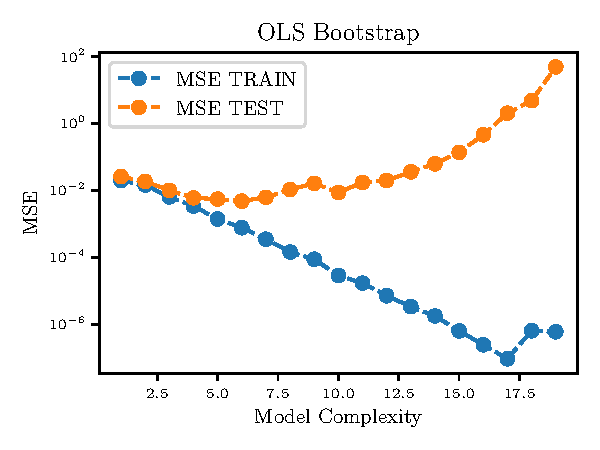
\includegraphics[width=\columnwidth]{../figs/OLS_MSE_Bootstrap_Hastie_211.pdf}
        \caption{\label{fig:Hastie2.11 MSE Bootstrap}The mean MSE for testing and training data with a 1/4 split resampled 500 times with bootstrap for a OLS regression of 300 randomly sampled points of the Franke Function.}
    \end{figure}

%\section{Discussion}

\section{Conclusion}

\onecolumngrid
\bibliography{bibfile}
\newpage
\twocolumngrid
\appendix


\end{document}
